\chapter{FaceItTools}
\section{Introduzione alla piattaforma}
\textit{FaceitTools.com} è una piattaforma di Larning Analytics sviluppata da un team di studenti provenienti da varie università del mondo, tra cui anche alcuni dell'Università di Padova che mette a disposizione dei corsi di varie materie universitarie strutturati principalmente in spidergram.
L'obiettivo è di facilitare l'apprendimento e mettere in evidenza come i corsi siano collegati tra loro, fornendo dei quiz sui quali si può essere valutati dai docenti.
\\Offre inoltre un sistema di raccolta feedback su domande d'esame archiviate in un database MongoDB che l’utente può cercare e filtrare usando una tabella Bootstrap.
\\Sulla base dei feedback viene effettuata un'analisi della difficoltà delle domande, infatti una volta inviate le risposte alle domande, viene visualizzato attraverso un grafico a barre il numero di risposte inviate e la difficoltà media percepita.
\\Questi feedback non sono utili solo agli studenti, ma anche ai docenti che possono capire se i corsi necessitano di essere rimodellati per essere più efficaci.
\begin{figure}[h]
    \centering
    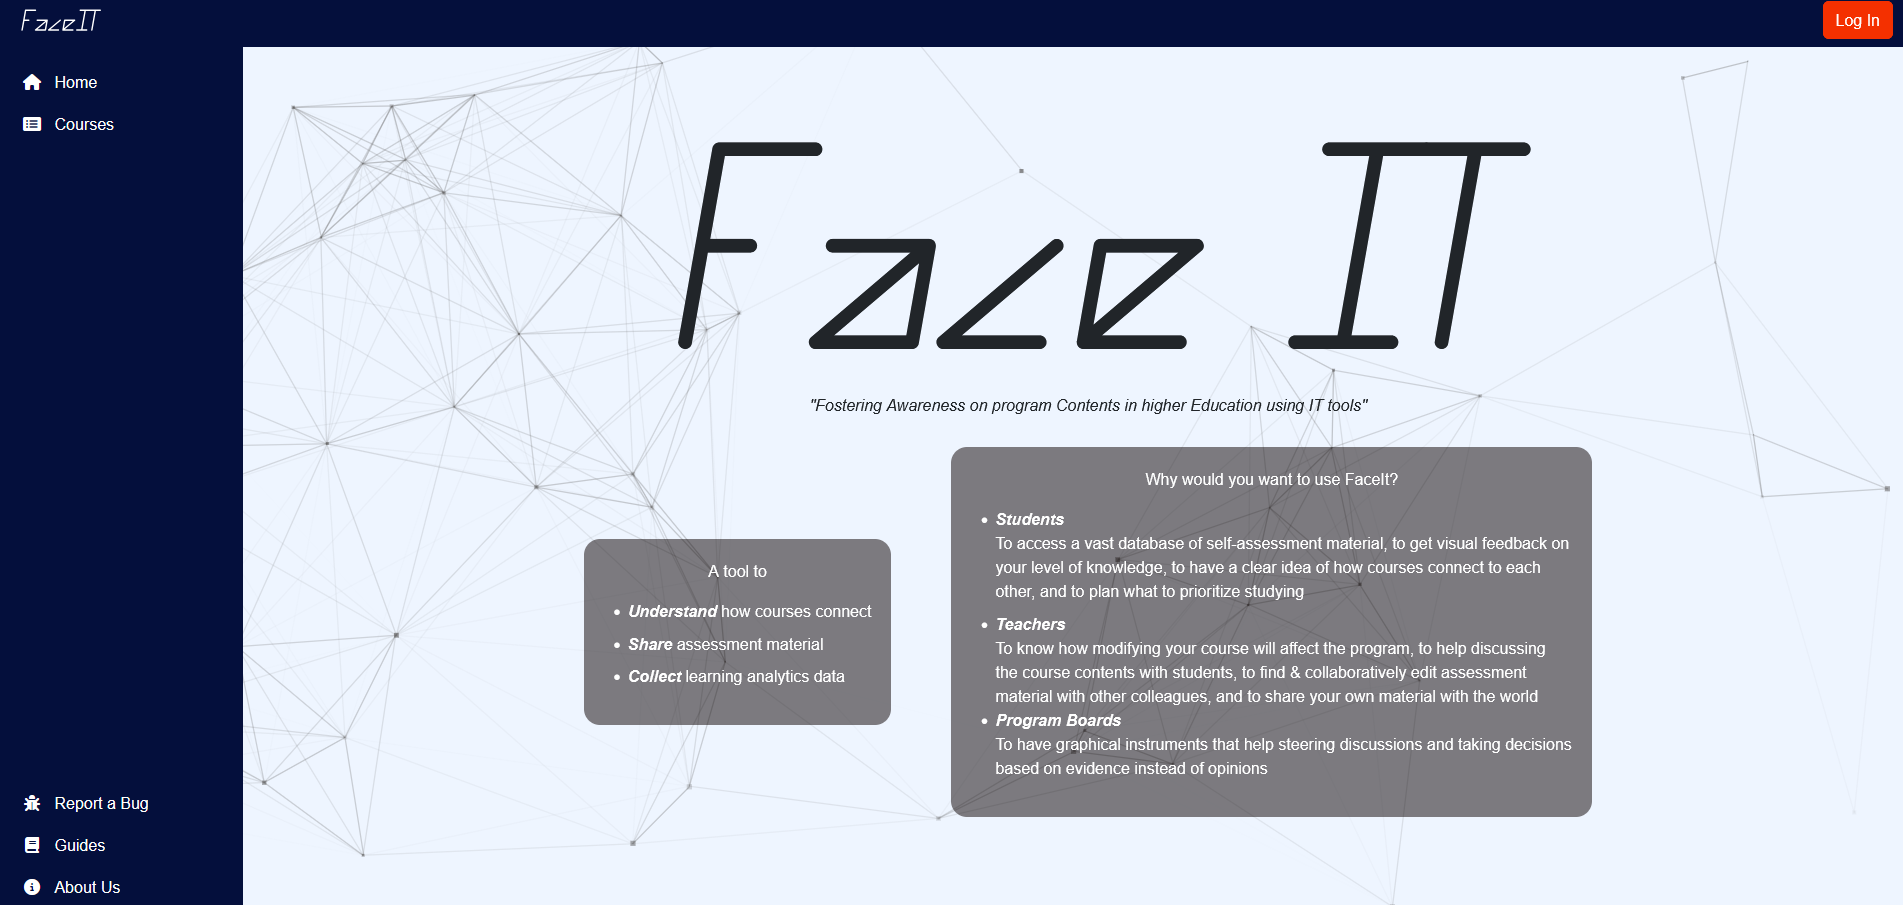
\includegraphics[width=0.65\textwidth]{Immagini/FaceItTools.PNG}
    \caption{FaceItTools homepage}
\end{figure}
\subsection{Ananlisi delle problematiche}
FaceItTools presenta le medesime problematiche affrontate nei capitoli precedenti riguardo le piattaforme centralizzate.
Nello specifico è priva di un sistema che sia in grado di verificare che i dati inseriti siano validi, ma soprattutto che appartengano ad utenti autorizzati.
\\Inoltre, problema ancor più grande, è la completa assenza di un sistema che vada a garantire la privacy degli studenti che condividono i loro dati, 
infatti è importantissimo garantire che solo chi ha diritto di accedere a quest'ultimi lo possa fare, tenendo anche traccia di chi lo fa e con che scopo.
\\Infine allo stato attuale del sito non è neanche possibile garantire che i dati non siano stati modificati violando le regole del sistema.
\subsection{Benefici di una trasformazione blockchain-oriented}
Una trasformazione blockchain-oriented della piattaforma FaceItTools porterebbe diversi benefici, 
il primo dei quali sarebbe in termini di privacy e sicurezza dei dati, in quanto gli studenti avrebbero il controllo totale sui propri dati di apprendimento.
\\Inoltre si guadagnerebbe anche nell'ambito della decentralizzazione, infatti grazie a ciò nessun singolo ente avrebbe il controllo sui dati.
\\Infine si avrebbe un miglioramento in termini di efficienza, dato che si accederebbe più velocemente ai dati grazie ad un Index Contract.
\newpage
\section{Raccomandazioni per gli sviluppatori}
\subsection{Modello di catena ibrido}
In questa sezione verranno fornite delle raccomandazioni e pseudo istruzioni per gli sviluppatori che vogliono implementare una trasformazione blockchain-oriented della piattaforma FaceItTools.
\\Una prima considerazione fondamentale da fare è quella che ci porterà poi a scegliere quale modello di catena è più adatto a questo caso.
Essendo che la prima cosa da andare a rispettare è la privacy dei dati e dei feedback degli studenti, 
il modello di catena più adatto sarà un ibrido tra il modello permiossioned e permissionless.
\\Questo perchè l'accesso deve esssere regolamentato e controllato, ma allo stesso tempo non deve essere centralizzato.
Abbiamo bisogno che non tutti i nodi possano accedere ai dati, ma solo quelli autorizzati e che gli studenti non gestiscano direttamente un nodo ma devono passare attraverso un provider,
in questo modo  si evita che gli studenti siano obbligati ad avere hardware dedicato e conoscenze tecniche e che inoltre venga impedito loro di manipolare i dati, questo perchè
i learning provider possono garantire sicurezza e protezione dei dati, seguendo standard elevati.
\\I dati sensibili devono essere conservati all'esterno della catena, quest'ultima si deve occupare solo di puntatori e hash crittografici.
\\Queste istruzioni sono tutte caratteristiche di una blockchain permissioned, ora però vediamo quali sono i requisiti derivanti dalla blockchain permissionless, in modo tale da avere il quadro completo sul perchè la blockchain risultante sarà ibrida.
La nostra blockchain dovrà essere chiaramente Ethereum-based e quindi sfruttare l'algoritmo di validazione PoS, perchè è l'unico modo che si ha per implementare gli Smart Contracts
che saranno protagonisti indiscussi del nostro sistema, in quanto rappresenteranno il tramite principale tra i dati sensibili e gli usufruitori degli stessi.
\subsection{Struttura dettagliata}
La struttura che viene fornita qui sotto prende spunto da quella presentata nel 2018 nell'articolo \textit{Connecting Decentralized Learning Records: A Blockchain Based
Learning Analytics Platform} \cite{ocheja2018connecting}, in quanto presenta le caratteristiche che si adattano al meglio al nostro caso di studio.
\begin{figure}[h]
    \centering
    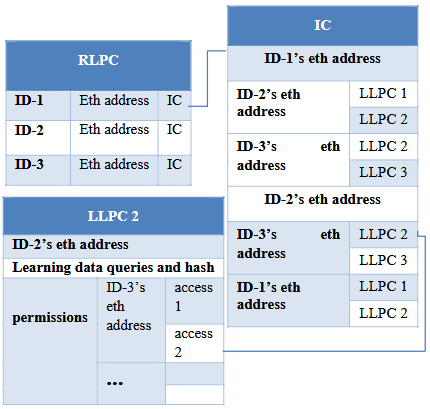
\includegraphics[width=0.65\textwidth]{Immagini/SmartContractsFaceIT.PNG}
    \caption{Interazione degli Smart Contracts nella Blockchain di FaceItTools}
\end{figure}
\\Nello specifico la Blockchain di FaceItTools sarà gestita da 3 smart contract:
\begin{enumerate}
    \item RLPC (Registrar – Learning Provider Contract) $\rightarrow$ regola l’accesso dei provider alla blockchain, controllando che siano autorizzati prima di farli entrare. Può utilizzare ID speciali o Token per verificarne la loro identità. In questo modo si garantisce che solo istituzioni verificate e riconosciute possono partecipare;
    \item LLPC (Learner – Learning Provider Contract) $\rightarrow$ rappresenta il legame tra lo studente e il provider, indicando dove sono i suoi dati;
          \\Esso contiene:
            \begin{itemize}
                \item il nome dello studente e l'indirizzo del database del provider;
                \item l’hash crittografico dei dati, per verificare che non siano stati modificati;
                \item le query che il provider può eseguire per recuperare i dati;
                \item la lista di permessi di accesso, gestita dallo studente;
            \end{itemize}
            \'E fondamentale in quanto consente ai dati reali di restare nel database del provider e non nella Blockchain, andando a proteggere la privacy degli studenti;
    \item IC (Index Contract) $\rightarrow$ Un indice globale che collega studenti, provider e i loro contratti per facilitare le ricerche.
            \\\'E organizzato in due Hash Table:
            \begin{itemize}
                \item Mappa Studenti $\rightarrow$ LLPC (ogni studente vede i suoi contratti);
                \item Mappa Provider $\rightarrow$ LLPC (ogni provider vede i contratti con gli studenti e con altri provider);
            \end{itemize}
            \'E importante perchè, se un provider vuole accedere ai dati di uno studente da un altro provider, viene creata una richiesta che deve essere approvata dallo studente, quindi funziona come un registro globale che collega studenti provider e dati, garantendo sicurezza e trasparenza.
\end{enumerate}